\chapter{Fine-grained Deduplication Technique using Program Contexts} 
\label{chap:FineDedup}

\section{Overview}
As the price-per-byte of NAND flash memory is rapidly decreasing,
NAND flash-based solid-state drives (SSDs) are emerging as a viable high-performance storage solution
for laptops, desktop PCs and high-performance enterprise systems.
However, as NAND flash memory technology scales down to 20-nm and below~\cite{tlc}, storing data reliably in NAND flash memory
gets a key design challenge of NAND-based storage systems. 
%For example, the number of program/erase (P/E) cycles allowed for each block is significantly reduced in recent triple-level cell (TLC)
%NAND technology.
%While older 5x-nm single-level cell (SLC) NAND flash memory can support about 10 K P/E cycles, recent 2x-nm TLC NAND flash memory
%can barely support about 1 K P/E cycles~\cite{tlc}.
Particulary, the reduction in the number of P/E cycles of NAND flash memory seriously limits the overall lifetime of flash-based SSDs,
making it difficult for SSDs to be used in write-intensive applications.

In order to extend the lifetime of flash-based SSDs,
data deduplication techniques have been used in recent SSDs
because they are effective in reducing the amount of data written to flash memory by preventing duplicate data 
from being written again~\cite{caftl,value-locality}.
As a result, only non-duplicate data, i.e., unique data, are stored in SSDs, thus effectively decreasing the total amount of data written to
SSDs.
In most deduplication schemes proposed for SSDs,
the unit of data deduplication is the same as the flash page size which is usually 4 KB or 8 KB.
%Using a page as a deduplication unit seems to be reasonable 
%because the unit of a read or write operation of flash memory is also a page. 
However, this page-based deduplication technique misses many chances of eliminating duplicate data, especially
when two pages are \textit{almost} identical.
%For example, in our experimental analysis of an existing 4 KB page-based deduplication technique, we observed that
%up to 34\% mostly identical data.
%If the unit of deduplication were smaller than 4 KB, about 23\% more data could be identified as duplicate data.
Furthermore, it is expected that the effectiveness of the page-based deduplication technique would 
get even worse in future NAND flash memory as the page size of 
flash memory is expected to increase
to a bigger size such as 16 KB~\cite{16kpage}.

In this dissertation, 
we propose a fine-grained deduplication technique for flash-based SSDs, called \textit{FineDedup}.
The proposed FineDedup technique is different from other existing deduplication techniques
in that it increases the likelihood of finding duplicates
by using a finer deduplication unit
which is smaller than a single page (e.g., one fourth of a single page).
With a smaller deduplication unit,
many data segments within a page can be detected as a duplicate one, 
so the amount of data written to flash memory can be reduced regardless of a physical page size.

In order to effectively incorporate fine-grained deduplication into flash-based SSDs,
two key technical issues must be addressed properly.
First, fine-grained deduplication requires a larger memory space than a coarse-grained one 
because it needs to keep more metadata in memory to find small-size duplicate data.
Second, in fine-grained deduplication, 
unique data segments from partially duplicated pages can be scattered across several physical pages,
which may seriously degrade the overall read performance.
The proposed FineDedup technique is designed to take full advantage of fine-grained deduplication
with small memory overhead as well as a low read performance penalty.
Our evaluation results show that 
FineDedup prolongs the lifetime of SSDs by up to 24\% over page-based deduplication
while requiring a negligible memory space increase.
This improvement comes with a less than 5\% read performance penalty over page-based deduplication.

\section{Selective Deduplication using Program Contexts}
As analyzed in Section~\ref{sec:duplicateactivity}, data duplicate patterns and I/O activities seems to
have relationship. 
Particulary, some writes are known a priori
to be likely to be unique. Applications might generate
data that should not or cannot be deduplicated. For
example, some applications write random, compressed,
or encrypted data; others write complex formats (e.g.,
virtual disk images) with internal metadata that tends to
be unique.

Attempting to deduplicate unique writes wastes CPU
time on hash computation and I/O bandwidth on maintaining
the hash index. Unique hashes also increase the
index size, requiring more RAM space and bandwidth
for lookup, insertion, and garbage collection.

In summary, if program context can help to
know when it is unwise to deduplicate a write, we can optimize
its performance and reliability. We implemented
a selective deduplication based on the program context.

Since deduplication uses computational resources
and may increase latency, it should only be performed
when there is a potential benefit. The program context
hint instructs the device not to deduplicate a particular
writes. It has two use cases:
(1) unique data: there is no point in wasting resources
on deduplicating data that is unlikely to have duplicates,
such as short-lived data; (2) reliability: maintaining
multiple copies of certain writes may be necessary,
e.g., superblock replicas in many file systems.

\begin{figure}[t]
	\center
	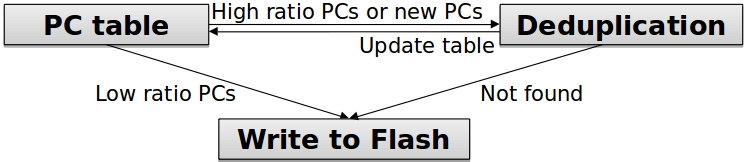
\includegraphics[scale=0.3]{figure/finededup/selectivededup}
	\caption{Diagram of selective deduplication.} % ok
	\label{fig:selectivededup}
\end{figure}

Figure~\ref{fig:selectivededup} shows a diagram of the proposed selective
deduplication technique. 
When a write request comes, it first query its PC value to the PC table which holds 
duplicate rate per PCs.
If the PC has high duplicate ratio or a new one, we apply deduplication on the request.
After fingerprinting and searching, the result is updated to the PC table.
If the PC has low duplicate ratio or there is no written data for a new PC,
we handle data as a normal reqeust.


\section{Exploiting Small Chunk Size }
\label{sec:finededup_motivation}

The write-requested page is identified whether the contents of the page have already been written and 
is written to flash memory only if there is no existing duplicate page. 
When a write-requested page is the exact duplicate of a previously written page, 
the requested page is not written to flash memory; 
only the corresponding entry for a mapping table (between the logical address and physical address) is updated. 
On the other hand, if there is no existing page duplicate in flash memory whose contents are the 
same as those of requested one, the requested page has to be written to flash memory. 
However, even for these unique pages, if their redundancy is checked at a sub-page level, 
say at a quarter of the page size, many sub-pages of these unique pages can be identified as redundant data. 
In existing techniques based on page-level deduplication, therefore, 
many duplicate data are written to flash memory even though the same data chunks have already been written.

In order to better understand the effect of fine-grained deduplication on the amount of identified duplicate data,
we analyzed how many more chunks can be identified as redundant 
when the chunk size gets smaller than a single page.
For our evaluation, we used four I/O traces, \texttt{RocksDB}, \texttt{GCC+cp}, \texttt{PC usage}, and \texttt{Package Tool} which are 
explained in Section~\ref{sec:finededup_experimentalresult}.
%collected from a desktop PC and a number of server systems used for a hardware synthesis, and a sensor data analysis.
In our evaluation, the page size was 4 KB and the chunk size was set to 1 KB.

\begin{figure}[t]
	\center
	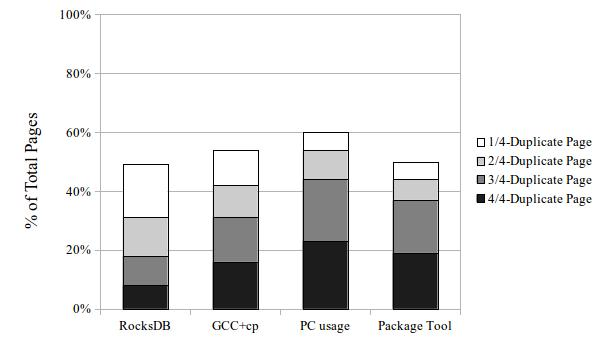
\includegraphics[scale=0.5]{figure/finededup/dupChunkperReq_}
	\caption{The percentage of pages according to their partial duplicate patterns.} % ok
	\label{fig:percentage}
\end{figure}

Fig.~\ref{fig:percentage} shows the percentage of the page writes from host, classified by their partial duplicate patterns.
We denote that a page is a n/4-duplicate page when n chunks of the page are duplicate chunks.
A 4/4-duplicate page is a duplicate page at the page level.
In the existing page-based deduplication, only 4/4-duplicate pages can be identified as a duplicate page.
As shown in Fig.~\ref{fig:percentage}, 4/4-duplicate pages account for only 8\% - 28\% of total requested pages.
%However, for partially duplicate pages where the number of duplicate chunks within a requested page is between 1 and 3,
For partially duplicate pages, i.e., 1/4-, 2/4- and 3/4-duplicate pages, the page-based deduplication technique is useless.
As shown in Fig.~\ref{fig:percentage},
pages with 1-3 duplicate chunks account for 14\% - 34\%.
This means that many duplicate data are unnecessarily written to flash memory
due to the large chunk size.
%when the size of a chunk is large.

\begin{figure}[t]
	\center
	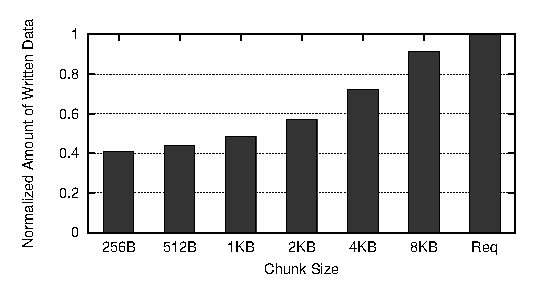
\includegraphics[scale=1]{figure/finededup/nonDuplicatedData_ChunkSize}
	\caption{The amount of written data under varying chunk sizes in \texttt{PC} workload.} % ok
	\label{fig:chunksize}
\end{figure}

We also investigated the amount of data that can be eliminated by data deduplication 
while varying the chunk size from 256 B to 8 KB.
As shown in Fig.~\ref{fig:chunksize}, 
when the chunk size is 1 KB, 
the amount of data written to flash memory is reduced by 33\% over when the chunk size is 4 KB.
In particular, when the size of a chunk is 8 KB (i.e., when the physical page size is assumed to be 8 KB),
only 10\% of requested data are eliminated by data deduplication.
This effectively shows that, as the size of a page increases,
the overall deduplication ratio, i.e., the percentage of identified duplicate writes, decreases significantly.
Since the physical page size of NAND flash memory is expected to increase as the semiconductor process is scaled down~\cite{tlc,16kpage},
it is expected that the deduplication ratio of the existing deduplication technique will be significantly 
decreased in near future.
In order to resolve this problem, the deduplication chunk size of deduplication techniques needs to be smaller than a page size.
As depicted in Fig.~\ref{fig:chunksize}, 
the deduplication ratio is saturated when the chunk size is 1 KB.
Thus, we use it as a default chunk size in the rest of this dissertation.



\section{Fine-Grained Deduplication}
\label{sec:finededup_finededup}
In order to effectively incorporate fine-grained deduplication into flash-based SSDs,
two key technical issues must be addressed properly.
First, fine-grained deduplication requires a larger memory space than a coarse-grained one 
because it needs to keep more metadata in memory to find small-size duplicate data.
Second, in fine-grained deduplication, 
unique data segments from partially duplicated pages can be scattered across several physical pages,
which may seriously degrade the overall read performance.
The proposed FineDedup technique is designed to take full advantage of fine-grained deduplication
with small memory overhead as well as a low read performance penalty.

In this section, we describe our proposed FineDedup technique in detail.
We first explain the overall architecture of FineDedup and 
describe how FineDedup handles read and write requests in Section~\ref{sec:finededup_architecture}.
In Section~\ref{sec:finededup_readoverheadmanagement} and ~\ref{sec:finededup_memoryoverheadmanagement}
we introduce a read performance penalty and memory overheads caused by FineDedup, respectively,
and explain how these problems can be resolved in FineDedup.

\subsection{Overall Architecture of FineDedup}
\label{sec:finededup_architecture}

Fig.~\ref{fig:overview} shows an overall architecture of FineDedup with its main components.
Upon the arrival of a write request,
FineDedup stores requested data temporarily in an on-device buffer,
which is managed by an LRU algorithm.
When the requested data are evicted from the buffer,
FineDedup divides the data into several chunks.
(Note that the chunk size is 1 KB in this work, 
but a different size of chunks can be used as well in FineDedup.)

For each chunk, FineDedup computes a fingerprint, using a collision-resistant hash function.
In this work, we use an MD6 hash function~\cite{md6}, which is one of the well-known cryptographic hash functions.
A fingerprint is used as a unique ID that represents the contents of a chunk.
FineDedup has to compute more fingerprints than the existing deduplication schemes
because of its small chunk size.
To reduce the hash calculation time,
FineDedup uses multiple hardware-assisted hash engines for parallel hash calculations. 
In our FPGA (ML605) implementation of the MD6 hash function, it took about 10 $\mu$s to compute a fingerprint using a hardware accelerator.
Considering a long write latency (e.g., 1.2 $m$s) of NAND flash memory,
the time overhead of computing fingerprints can be considered negligible.

After fingerprinting, 
each fingerprint is looked up in the dedup table
which maintains the fingerprints of the unique chunks previously written to flash memory.
Each entry of the dedup table is composed of a key-value pair, \{\textit{fingerprint}, \textit{location}\},
where the location indicates a physical address in which the unique chunk is stored.
If the same fingerprint is found,
it is not necessary to write the chunk data
because the same chunk is already stored in flash memory.
Instead, FineDedup updates the mapping table 
so that the corresponding mapping entry points to the unique chunk previously written.
Unlike existing page-based deduplication techniques,
FineDedup handles all the data in the unit of a chunk.
%For this reason, FineDedup must maintain a chunk-level mapping table,
%which is much larger than the existing page-level mapping table.
For this reason, FineDedup must maintain a chunk-level mapping table
that maps a logical chunk address to a physical chunk in flash memory.
Because of its finer mapping granularity,
the chunk-level mapping table is much larger than the existing page-level mapping table.
To reduce the memory space for maintaining the chunk-level mapping table,
FineDedup uses a hybrid mapping strategy,
which is described in Section~\ref{sec:finededup_memoryoverheadmanagement} in detail.

\begin{figure}[t]
	\center
	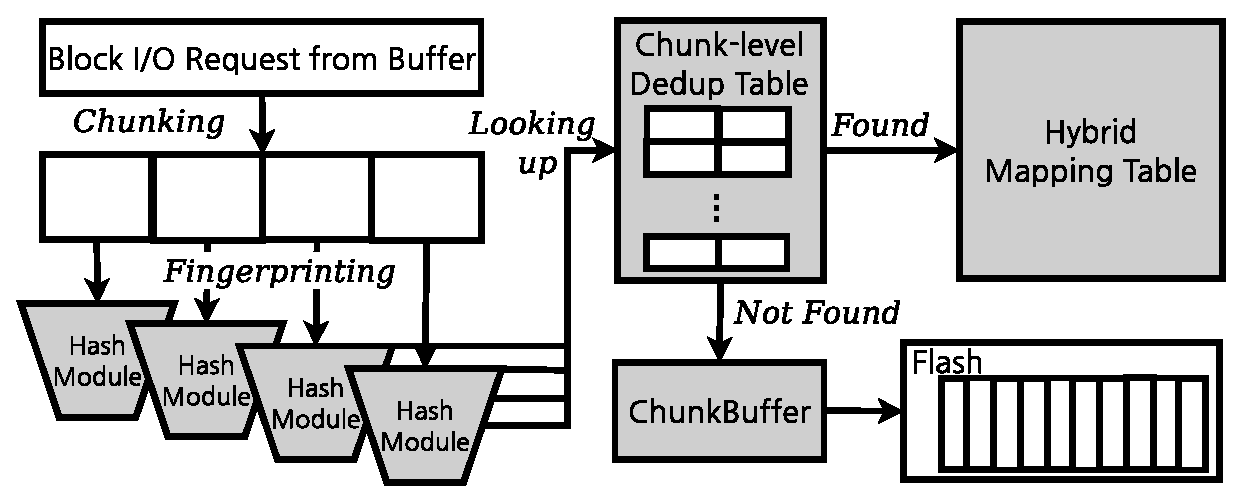
\includegraphics[scale=0.4]{figure/finededup/overview}
	\caption{An overview of the proposed FineDedup technique.} % ok
	\label{fig:overview}
\end{figure}

If there is no matched fingerprint in the dedup table,
FineDedup stores the chunk data in a \textit{chunk buffer} temporarily.
This temporary buffering is necessary 
because the unit of I/O operations of flash memory is a single page.
The chunk buffer stores the incoming chunk data until there are four chunks,
and evicts them to flash memory at once.
FineDedup then updates the mapping table 
so that the corresponding mapping entries indicate newly written chunks.
The new fingerprints of the evicted chunks are finally inserted into the dedup table with their physical location.

When a read request arrives,
FineDedup reads all the chunks that belong to the requested page from flash memory,
and then transfers the read data to the host system.
The physical addresses of the chunks can be obtained by consulting to the mapping table.
In FineDedup, four chunks in the same logical page can be scattered across different physical pages.
In that case, multiple read operations are required to form the original page data,
which in turn significantly increases the overall read response time.
We explain how FineDedup resolves this problem in the following subsection.

\subsection{Read Overhead Management}
\label{sec:finededup_readoverheadmanagement}

FineDedup effectively reduces the number of pages written to flash memory
by using a small-size chunk for deduplication,
but it incurs two types of additional overheads, i.e.,
a read performance overhead and a memory space overhead,
which are not observed in the existing deduplication techniques.
In this subsection, 
we first introduce why the read performance overhead occurs in FineDedup,
and then explain how FineDedup resolves this problem.
In the following subsection, 
we describe our memory space overhead reduction technique in detail.

The main cause of the read performance degradation is data fragmentation
which occurs when data chunks belonging to the same logical page are broken up into several physical pages.
Fig.~\ref{fig:readoverhead} illustrates why data fragmentation occurs in FineDedup.
There are two page write requests, \textit{Req 1} and \textit{Req 2}, in Fig.~\ref{fig:readoverhead}.
\textit{Req 1} consists of four chunks, `A', `B', `C', and `D', 
and \textit{Req 2} is also composed of four chunks, `E', `F', `G', and `H'.
Since `A' and `B' of \textit{Req 1} are duplicate chunks,
only `C' and `D' need to be written to flash memory.
%Thus, we can reduce writes for two chunks `A' and `B'.
Suppose that there is a read request for the page data written by \textit{Req 1}.
%after the chunks of \textit{Req1} are written to flash memory.
In that case, FineDedup has to read three pages, i.e., \textit{page 1}, \textit{page 2}, and \textit{page 3}, from flash memory
to form the requested data.
%to form the requested data of \textit{Req1}, incurring a significant read performance penalty.
The read performance penalty can also occur even when there are no duplicate chunks in the requested page.
For example, in Fig.~\ref{fig:readoverhead}, 
\textit{Req 2} has no duplicate chunks in flash memory,
thus all the chunks belonging to \textit{Req 2} being written to flash memory.
Because a single page write requires four data chunks, 
`E' and `F' of \textit{Req 2} are written to \textit{page 3} together with `C' and `D',
and `G' and `H' will be written to \textit{page 4} with other data chunks, as shown in Fig.~\ref{fig:readoverhead}.
Thus, when the data written by \textit{Req 2} are read later, 
both \textit{page 3} and \textit{page 4} must be read from flash memory.

\begin{figure}[t]
	\center
	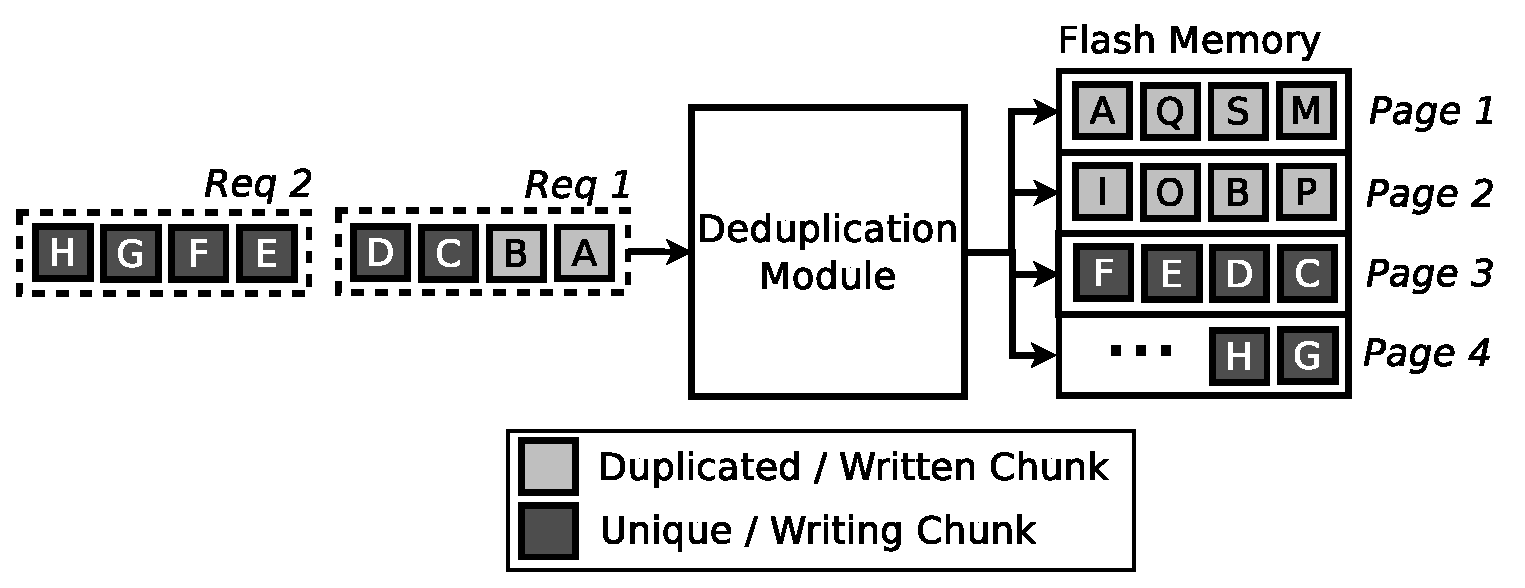
\includegraphics[scale=0.4]{figure/finededup/readoverhead}
	\caption{Data fragmentation caused by FineDedup.} % ok
	\label{fig:readoverhead}
\end{figure}


One of the feasible approaches that mitigate the read performance overhead is to employ a chunk read buffer.
In our observation, 
the access frequencies of unique chunks are greatly skewed;
that is, a small number of popular chunks account for a large fraction of the total accesses to unique chunks in flash memory.
For example, according to our analysis under real-world workloads, 
top 10\% of the unique chunks serve more than 70\% of the total data read by a host system.
By keeping frequently accessed chunks in a chunk read buffer,
therefore, FineDedup can reduce a large number of page read operations sent to flash memory.

\begin{figure}[t]
	\center
	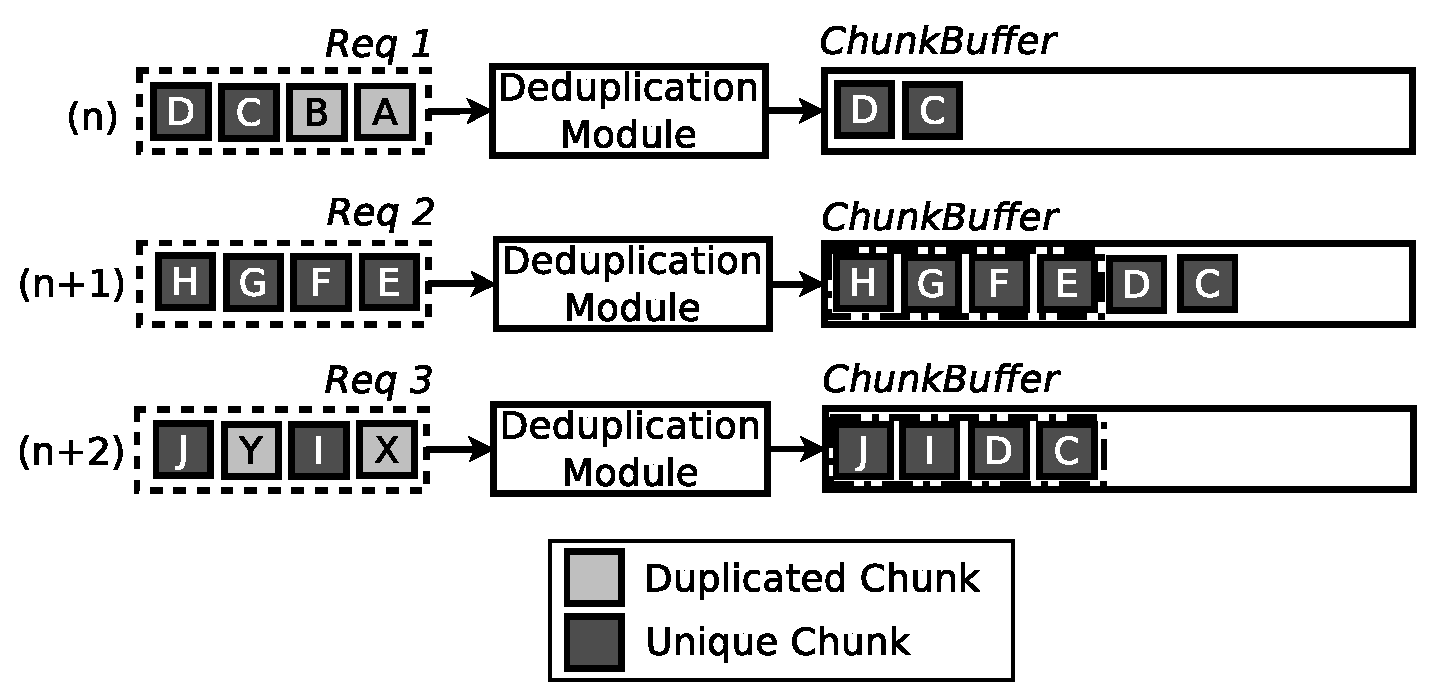
\includegraphics[scale=0.4]{figure/finededup/chunkbuffer}
	\caption{A packing scheme in the \textit{chunk buffer}.} % ok
	\label{fig:chunkbuffer}
\end{figure}

On the other hands, we have observed that about 39\% of read requests to unique pages actually requires two page read operations.
In order to further reduce this read performance penalty,
FineDedup uses a chunk packing scheme.
The key idea of this scheme is to
group chunks belonging to the same logical page in a chunk buffer and 
then write them to the same physical page together.
Fig.~\ref{fig:chunkbuffer} shows an example of our chunk packing scheme
when three page write requests, \textit{Req 1}, \textit{Req 2}, and \textit{Req 3}, are consecutively issued from a host system.
\textit{Req 1} contains two duplicate chunks `A' and `B' and two unique chunks `C' and `D'.
As expected, only `C' and `D' out of four chunks are sent to the chunk buffer.
The next request \textit{Req 2} does not have any duplicate chunks,
so all of them are moved to the chunk buffer.
As depicted in Fig.~\ref{fig:chunkbuffer},
the chunks `E', `F', `G', and `H' belong to the same logical page and form single page data.
Thus, FineDedup writes them to flash memory together,
leaving the chunks `C' and `D' in the chunk buffer.
When \textit{Req 3} is issued with two more unique chunks `I' and `J', 
`C' and `D' along with `I' and `J' are written to flash memory.
All those chunks can be written to the same physical page together
because every chunk of each request is not broken up into two pages.

Note that the main objective of this scheme is to prevent chunks of a unique request to be scattered across multiple pages 
avoiding unnecessary data fragmentation.
In order to directly insert a incoming unique request to chunk buffer,
page-sized free space is managed to be always available in the buffer.
When there is no free space for the next request and no suitable chunks of requests to form a single page,
the chunks of a partially duplicate request is broken up into two pages.
Most partially duplicated requests, however, are 3/4-Duplicate pages as shown in Fig.~\ref{fig:percentage}, which means 
there are many requests of one unique chunk in the chunk buffer.
Therefore, we can expect that most requests will be written to the same page even when the size of the chunk buffer is not large 
since it is not quite difficult to find an appropriate chunk to fit a flash page.
In the above example, if we assume the chunk buffer can contain 8 chunks and \textit{Req 3} has three unique chunks,
only two chunks of \textit{Req 3} will be written along with existing chunks, `C' and `D', leaving the other chunk in chunk buffer.
A large chunk buffer provides more chance to avoid the request scattering.


%%%%% NEED TO BE EXPLAINED!!! POWER FAILURE 시 partial chunks 'C', 'D' 가 power-off recovery 될 수 있음. => reliability 관리  %%%
Remaining data in the chunk buffer could be lost when a power failure occurs.
Recent enterprise SSDs, such as SM825 model manufactured by Samsung, have a large SDRAM cache (e.g., 256 - 512 MB) and use it as a device buffer.
Moreover, they support internal cache power protection through the use of capacitors to flush out information in DRAM to flash memory 
at the event of power failure~\cite{sm825}.
In order to keep the reliability in FineDedup, the remaining data in the chunk buffer can be stored to flash memory 
during power protection procedure as well as the mapping information of the written page.
In conclusion for chunk buffer design, there is a trade-off between potential read performance 
and reliability depending on the chunk buffer size.
The size of the chunk buffer, hence, should be determined according to the characteristics of workloads.

\subsection{Memory Overhead Management}
\label{sec:finededup_memoryoverheadmanagement}

As mentioned in Section~\ref{sec:finededup_architecture},
FineDedup handles requested data in the unit of a chunk.
Therefore, FineDedup must maintain a chunk-level mapping table
that maps a logical chunk address to a physical chunk address in flash memory.
Since the size of a chunk is smaller than that of a page,
a chunk-level mapping table is much larger than the page-level mapping table.
For example, suppose that the page size is 4 KB and the chunk size is 1 KB.
In that case, the size of a chunk-level mapping table is four times larger than that of a page-level mapping table.

In order to reduce the amount of memory space required for a mapping table,
FineDedup employs a hybrid mapping table
which is composed of two types of mapping tables:
a page-level mapping table and a chunk-level mapping table.
As depicted in Fig.~\ref{fig:percentage}, 
duplicate pages and unique pages still account for a considerable proportion of the total written pages.
%for writing by a host system.
For these pages, the page-level mapping table is more appropriate 
because they can be directly mapped to corresponding pages in flash memory.
The chunk-level mapping table is required only for partially duplicate pages.

\begin{figure}[t]
	\center
	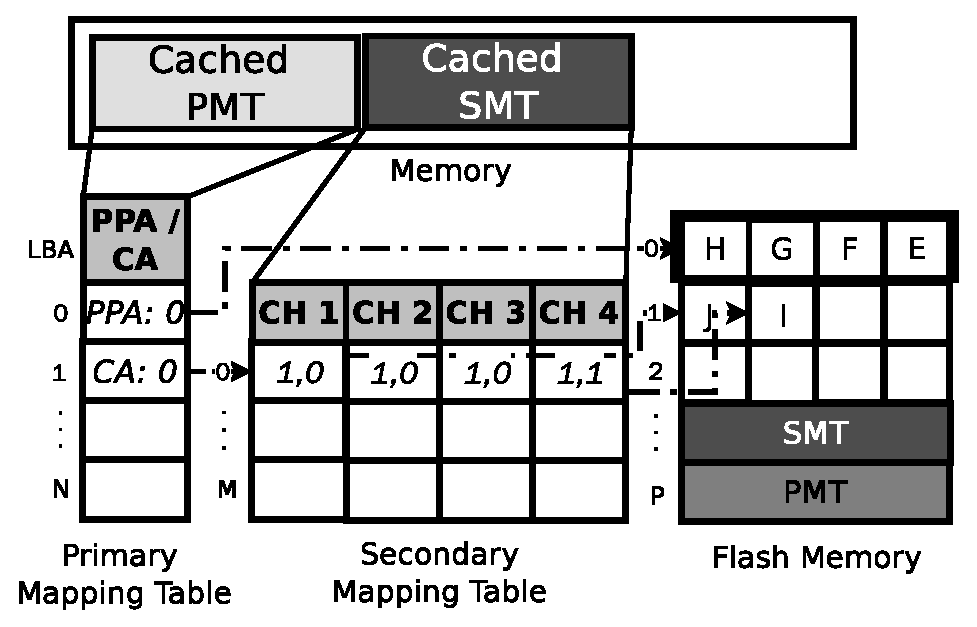
\includegraphics[scale=0.5]{figure/finededup/hybridmapping_1}
	\caption{An overview of the demand-based hybrid mapping table.} % ok
	\label{fig:hybridmapping}
\end{figure}


Fig.~\ref{fig:hybridmapping} shows the overall architecture of the hybrid mapping table used in FineDedup.
The primary mapping table (PMT) is maintained in the page level 
while the secondary mapping table (SMT) is maintained in the chunk level.
The entry of the PMT is either a physical page address (PPA in Fig.~\ref{fig:hybridmapping}) in flash memory or 
an index of the SMT (chunk address (CA) in Fig.~\ref{fig:hybridmapping}). 

%%%%%
%만약 request의 mapping 이 chunk 수준으로 관리될 필요가 없으면, 즉, unique page or fully duplicated page,  
If the chunk-level mapping is not necessary for a requested page, for example, unique page or duplicate page,
the corresponding entry of the PMT directly points to the physical address of the 
newly written page or existing unique page in flash memory, respectively.
%%%%%
%If the requested page is a duplicate one, 
%the corresponding entry of the primary mapping table directly points to the physical address of the existing unique page 
%in flash memory.
%Similarly, if the requested page is unique one, the corresponding entry of the primary mapping table is 
%updated to point to the newly written unique page.
%%%%
On the other hand, if a partially duplicate page is requested for writing, 
FineDedup allocates a new entry in the SMT.
As depicted in Fig.~\ref{fig:hybridmapping},
each entry of SMT is composed of four fields, each of which points to the physical chunk address 
in flash memory.
FineDedup then updates the new entry so that each field points to the physical chunk address.
The corresponding entry of the PMT indicates the newly allocated entry of the SMT.

Using the hybrid mapping table, 
FineDedup can reduce the amount of memory space for keeping a mapping table.
However, the problem of this hybrid mapping approach is that 
the size of a mapping table can greatly vary according to the characteristics of workloads.
For example, if some workloads have many partially duplicate pages, 
the size of the SMT gets too big.
On the other hand, if workloads mostly have unique pages or duplicate pages, 
the it can be very small.
Thus, the hybrid mapping table cannot be directly adopted in real SSD devices whose DRAM size is usually fixed.
To overcome such a limitation, 
FineDedup adopts a demand-based mapping strategy in which
the entire chunk-level mapping table is stored in flash memory
while caching only a fixed number of popular entries in DRAM memory.
The \textit{Cached PMT} and \textit{Cached SMT} in Fig.~\ref{fig:hybridmapping} represents the cached versions of the
PMT and SMT, respectively.

It has been known that the demand-based mapping requires extra page read and write operations~\cite{dftl}.
For instance,
if a mapping entry for a chunk to be read is not found in the in-memory mapping table,
that entry must be read from flash memory while evicting a victim entry to flash memory.
The temporal locality present in workload, however, helps keep the number of extra operations small.
The mapping information of requests issued in similar times will be stored in the same flash page.
Once a mapping page is loaded in memory, hence,
most requests issued in similar times are serviced from the mappings in memory.

\section{Experimental Results}
\label{sec:finededup_experimentalresult}

%In this section, 
%we first describe our experimental settings and explain the benchmarks used for our evaluation in detail.
%We then assess the effect of the proposed FineDedup technique on the SSD lifetime.
%Finally, we analyze the read performance penalty and the memory overhead caused by FineDedup.
%{\color{blue}We then analyze the benefit of the proposed FineDedup technique over the existing deduplication technique 
%in terms of the SSD lifetime and overheads such as the additional read operation and the required memory size.}


In order to evaluate the effectiveness of FineDedup, 
we performed our experiments using a trace-driven simulator with the I/O traces collected under various applications.
The trace-driven simulator modeled the basic operations of NAND flash memory, 
such as page read, page write and block erase operations,
and included several flash firmware algorithms, 
such as garbage collection and wear-leveling.
The proposed FineDedup technique and the existing deduplication techniques were also implemented in our simulator.

For trace collection, 
we modified the Linux kernel 2.6.32 and collected I/O traces at the level of a block device driver.
All the I/O traces include detailed information about the I/O commands sent to a storage device
(e.g., the type of requests, logical block addresses (LBA), the size of requests, etc.) 
as well as the contents of the data sent to or read from a storage device.
We recorded I/O traces while running various real-world applications.
The detailed descriptions of these I/O traces are summarized in Table~\ref{tab:traces}.

\begin{table}[t]
	\renewcommand{\tabcolsep}{1.4mm} 
	\centering
	\begin{tabular}{c|c|c|c}
		\hline
		\multirow{2}{*}{Trace} 		& \multirow{2}{*}{Description} 		& Amount of 	& Amount of \\
							   		& 			 				  		& Writes 		& Reads \\
		\hline
		\hline
		\multirow{2}{*}{\texttt{RocksDB}} 		& Benchmarking on the  & \multirow{2}{*}{3.1 GB} 	& \multirow{2}{*}{810 MB} \\
									   	   	    & Key-value store  		& 						 	& 						  \\
		\hline
		\multirow{2}{*}{\texttt{GCC+cp}}    	& Developing 		& \multirow{2}{*}{2.6 GB} 	& \multirow{2}{*}{66 MB} \\
											   	& Kernel modules  		& 							& 					   \\

		\hline
		\multirow{2}{*}{\texttt{PC usage}} 	   	& Web surfing, emailing and & \multirow{2}{*}{2.5 GB} 	& \multirow{2}{*}{70 MB} \\
											   	& editing document, etc. &   						& 						  \\

		\hline
		\multirow{2}{*}{\texttt{Package Tool}} 	 & Installing \& upgrading & \multirow{2}{*}{4.9 GB} 	& \multirow{2}{*}{119 MB} \\
										   	 & software packages			& 						   	& 					   \\
		\hline
	\end{tabular}
	\caption{A summary of traces used for experimental evaluations.}
	\label{tab:traces}
\end{table}


\subsection{Effectiveness of FineDedup}

\begin{figure}[t]
	\center
	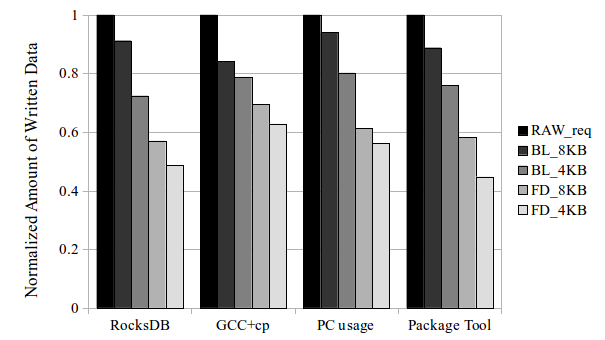
\includegraphics[scale=0.6]{figure/finededup/dataReduction_Chunksize_less_}
	\caption{The amount of written data under various schemes.} % ok
	\label{fig:reducedData}
\end{figure}


Fig.~\ref{fig:reducedData} shows the amount of data written to flash memory by FineDedup over the existing scheme.
The results shown in Fig.~\ref{fig:reducedData} are normalized to \textit{RAW\_req},
which represents the total amount of data written to flash memory without data deduplication.
We assume the page-based deduplication technique as a baseline case.
The baseline is denoted by \textit{BL\_4KB} for a 4 KB flash page and \textit{BL\_8KB} for a 8 KB flash page.
Our FineDedup technique is denoted by \textit{FD\_4KB} and \textit{FD\_8KB} for a 4 KB flash page and 
a 8 KB flash page, respectively.
The chunk size in FineDedup is set to 1 KB for a 4 KB flash page and 2 KB for a 8 KB flash page.

As we can see in Fig.~\ref{fig:reducedData}, 
the effectiveness of deduplication techniques is highly workload-dependent. 
The amount of data eliminated by the deduplication technique notably increases 
when FineDedup is applied in most of the traces except \texttt{M-media}.
%as the chunk size decreases in three traces, i.e., \texttt{PC}, \texttt{Sensor}, and \texttt{Synth}. 
When we set the chunk size to one fourth of the flash page size, 
FineDedup removes on average 16\% more duplicate data 
over \textit{BL\_4KB} for a 4 KB flash page.
For a 8 KB flash page, 
it removes more duplicate data, on average by 23\% over the existing technique.
For \texttt{RocksDB}, FineDedup saves 37\% flash writes over \textit{BL\_8K}.
As expected, the benefit of FineDedup mainly derives from the decreased chunk size 
because it increases the probability of finding and eliminating duplicate data.
Especially, \texttt{RocksDB} trace shows a large number of write requests with little different data during
compaction, so FineDedup can effectively 
identify unchanged data as duplicate while existing deduplication technique regards as unique data.

\subsection{Read Overhead Evaluation}
\label{sec:finededup_readoverheadevaluation}

\begin{figure}[t]
	\center
	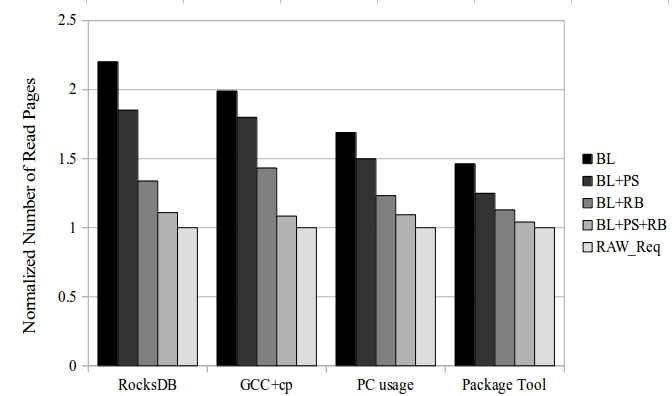
\includegraphics[scale=0.4]{figure/finededup/increasedPageRead_}
	\caption{The number of page read operations.} % ok
	\label{fig:pageread}
\end{figure}

As explained in Section~\ref{sec:finededup_readoverheadmanagement}, 
%subpage chunking in FineDedup increases the number of page read operations. 
fine-grained chunking in FineDedup increases the number of page read operations. 
%In FineDedup, we have have proposed the optimization techniques, such as the packing scheme and the chunk read buffer,
%to reduce additional page read operations.
Fig.~\ref{fig:pageread} shows the normalized number of page read operations compared with the number of read requests
in the workloads.
\textit{RAW\_Req} indicates the number of original page read requests and \textit{BL} refers to the number of page
read operations of the baseline FineDedup without employing proposed optimization schemes. 
\textit{BL+PS}, \textit{BL+RB} and \textit{BL+PS+RB} indicate the number of page reads of FineDedup with the proposed
packing scheme, the chunk read buffer, and both, respectively. 
The size of the chunk read buffer was set to 8 MB and the chunk buffer size was set to 200 KB.

As shown in Fig.~\ref{fig:pageread}, employing the chunk read buffer is more effective than the packing scheme 
for reducing additional page read operations in most workloads. This is because the packing scheme is only
effective for the requests containing no duplicate chunks whereas the chunk read buffer can absorb most of the read requests 
to frequently accessed chunks.
FineDedup with both the packing scheme and chunk read buffer incurs on average less than 5\% of additional read operations
over the existing deduplication technique.

\subsection{Memory Overhead Evaluation}
\label{sec:finededup_memoryoverheadevaluation}

As explained in Section~\ref{sec:finededup_memoryoverheadmanagement},
chunk level mapping table requires large memory space to handle partially duplicate pages.
In FineDedup, we have proposed 
the demand-based hybrid mapping table to reduce the required memory size for a mapping table without performance degradations.
In Fig.~\ref{fig:mappingoverhead}, the effectiveness of the proposed mapping table is evaluated in terms of the hit ratio and 
the amount of additional written data with various memory sizes for the cache.
Since the PMT of the hybrid mapping table in FineDeup is the same approach as the DFTL~\cite{dftl}, which is a well-known 
demand-based scheme to exploit the page-level mapping,
the overhead of PMT can be estimated from the overhead of DFTL.
Thus, in order to focus on the overhead of the SMT, we assume that DFTL is employed as the baseline mapping scheme in our evaluation.

\begin{figure}[t]
	\center
	\subfloat[Hit ratio of SMT cache]{\label{fig:mappingcachehit}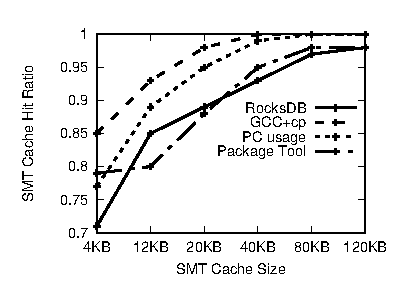
\includegraphics[scale=0.8]{figure/finededup/mappingcachehit_}}
	\subfloat[Extra data written due to SMT cache evictions]{\label{fig:mappingeviction}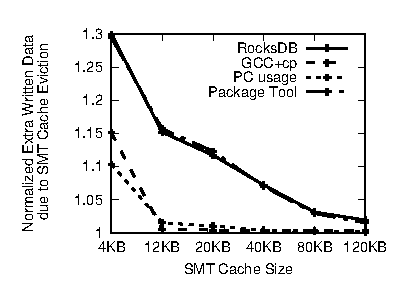
\includegraphics[scale=0.8]{figure/finededup/mappingeviction_}}
	\caption{The effectiveness of the demand-based hybrid mapping table in FineDedup with various cache sizes.}
	\label{fig:mappingoverhead}
\end{figure}

Fig.~\ref{fig:mappingoverhead}(a) shows the hit ratio of the cached SMT. 
With a 120 KB cache, more than 95\% of the mapping table accesses are absorbed.
In addition, Fig.~\ref{fig:mappingoverhead}(b) shows extra written data caused by the evicted page entries 
from the SMT cache.
Since mapping table accesses occur in the middle of read/write operations, it is important to reduce the 
amount of written data from evicted page entries in terms of read/write performance.
Similar to the hit ratio, the overhead by the eviction becomes almost negligible 
when the cache size is set to 120 KB under most workloads.
As a result, FineDedup does not incur a significant memory overhead 
even when the fine-grained chunking method is not effective.



\begin{comment}
\subsection{Evaluation of the Effectiveness of Cached Mapping Table for Mixed Workloads}

\begin{figure}[t]
	\center
	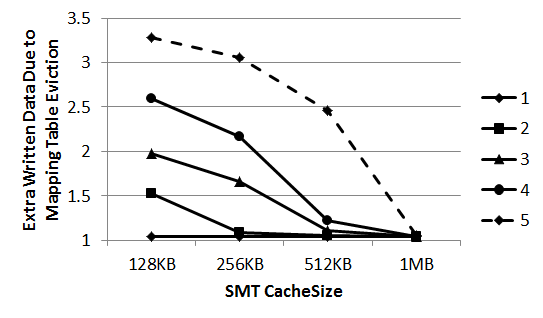
\includegraphics[scale=0.45]{figure/finededup/evicteddata_result.png}
	\caption{The amount of extra written data due to mapping table eviction for the mixed workload.} % ok
	\label{fig:eviction_mixed}
\end{figure}

The effectiveness of the cached mapping table is evaluated for mixed workloads. 
Fig.~\ref{fig:eviction_mixed} shows the normalized amount of additionally written data due to the 
mapping table eviction. 
The mixed traces are composed by accumulating individual traces in the order of 
\texttt{PC}, \texttt{Synth}, \texttt{Sensor}, \texttt{Install}, and \texttt{Update}. 
For example, mixed workload 4 is composed with \texttt{PC}, \texttt{Synth}, \texttt{Sensor}, and \texttt{Install}.
Although, the cached mapping table is not effective as the number of traces is increased, 
the performance degradation rate is smaller than the number of workload increasing rate. 
Moreover, mapping table caching will be effective when the caching memory is big enough to contain 
the working set of each trace. 
In the evaluation, the required memory space for the cached mapping table is about 1 MB for the mixed workload. 
Considering that commercial SSDs have hundreds of GBs of DRAM, the memory overhead of a few MB is not large.


\subsection{Evaluation of the Effectiveness of the Chunk Read Buffer}
\begin{figure}[t]
	\center
	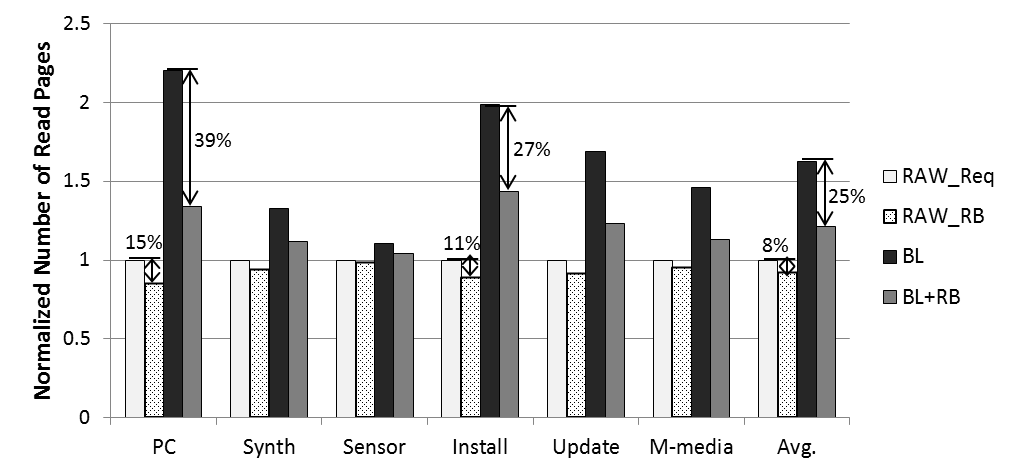
\includegraphics[scale=0.65]{figure/finededup/readbuffer_result.png}
	\caption{The number of page reads with and without read buffer.} % ok
	\label{fig:readbuffer}
\end{figure}

The effectiveness of the chunk read buffer between the baseline policy and FineDedup is evaluated. 
Fig.~\ref{fig:readbuffer} shows the amount of page reads for the baseline policy and FineDedup 
with and without the read buffer. 
The read buffer absorbs about 8\% read requests of \textit{RAW\_req}, whereas the read requests are 
reduced by about 25\% with the read buffer for FineDedup on average. 
Based on the analysis, the higher effectiveness of the read buffer in FineDedup is 
because of the increased memory utilization by deduplication. 
The read buffer in the baseline policy can absorb read requests for pages that have already been read. 
Chunk read buffer in FineDedup, however, can also absorb the read requests for deduplicated pages pointed 
by the hybrid mapping table. 
Therefore, with the same read buffer size, more read requests can be absorbed in FineDedup.


\subsection{Sensitivity Study on Chunk Read Buffer Size}
In addition to the evaluation of read overhead management shown in Section~\ref{sec:finededup_readoverheadevaluation},
we have evaluated that how the size of the chunk read buffer affects the number of read operations.
Fig.~\ref{fig:buffersize} shows the normalized number of read operations compared with the number
of read requests in the workloads while varying the buffer size from 8 KB to 32 MB.
The LRU scheme is used to be a replacement scheme in the chunk read buffer.
The chunk buffer is not used in this evaluation in order to focus only on the chunk read buffer.
When the buffer size gets larger, the number of read operations decreases.

\begin{figure}[t]
	\center
	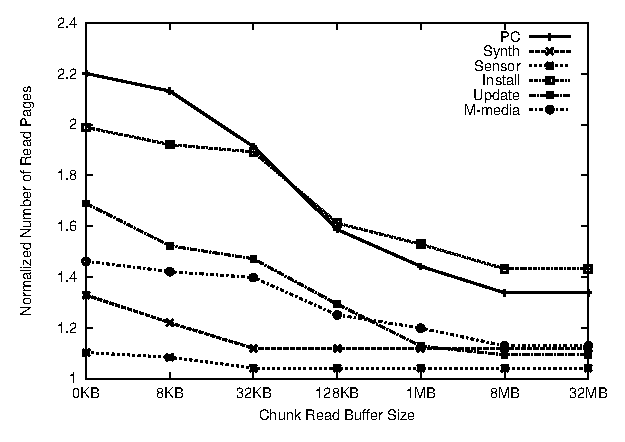
\includegraphics[scale=0.8]{figure/finededup/buffersize}
	\caption{The number of page read operations under varying chunk read buffer sizes.} % ok
	\label{fig:buffersize}
\end{figure}

As explained in Section~\ref{sec:finededup_readoverheadmanagement}, the access frequencies of unique chunks are greatly skewed.
Thus, it is important for read performance to keep those hot chunks in the chunk read buffer.
As shown in Fig.~\ref{fig:buffersize}, the chunk read buffer can absorb most read requests 
except for \texttt{PC} and \texttt{Install} traces.
In the \texttt{PC} and \texttt{Install} traces, 
the skewness of unique read accesses to hot chunks was significantly lower than other traces, thus
limiting the effectiveness of the chunk read buffer.
Since the effectiveness of the chunk read buffer diminishes as its size increases more than 8 MB,
in our experiments in Section~\ref{sec:finededup_readoverheadevaluation}, a 8 MB chunk read buffer was used.

\subsection{Sensitivity Study on Chunk Buffer Size}
\begin{figure}[t]
	\center
	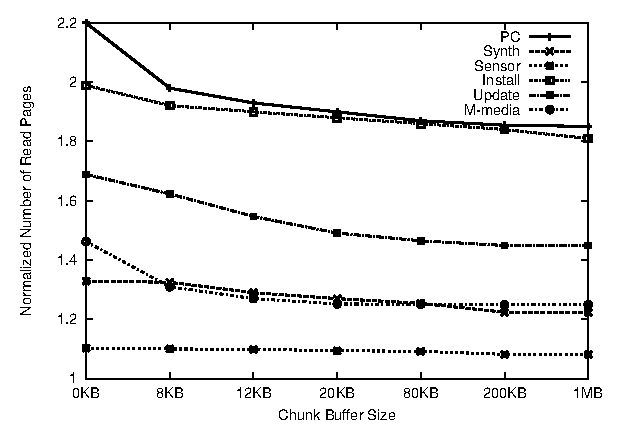
\includegraphics[scale=0.8]{figure/finededup/chunkbuffersize}
	\caption{The number of page read operations under varying chunk buffer sizes.} % ok
	\label{fig:chunkbuffersize}
\end{figure}


We have also evaluated that how the size of chunk buffer affects the number of read operations.
As explained in Section~\ref{sec:finededup_readoverheadmanagement},
the chunk buffer separates chunks of unique requests and chunks of partially duplicate requests.
Moreover, it also tries not to split chunks of partially duplicate requests into multiple pages.
Thus, a larger chunk buffer can reduce more potential extra read operations by preventing chunk splits.
Fig.~\ref{fig:chunkbuffersize} shows the normalized number of read operations compared with the number of read requests
in the workloads while varying the chunk buffer size from 8 KB to 1 MB.
For this evaluation, the chunk read buffer is not used to focus only on the chunk buffer.

As shown in Fig.~\ref{fig:chunkbuffersize}, the number of read operations does not decrease much as the chunk buffer size increases.
Since most partially duplicated requests in our traces is 3/4-Duplicate pages as explained
in Section~\ref{sec:finededup_readoverheadmanagement}, 
it is not difficult to find an appropriate chunk to fit a single flash page.
As shown in Fig.~\ref{fig:chunkbuffersize}, however, the benefit of chunk buffer is rather limited.
For example, there is no significant saving in the number of read pages for a chunk buffer larger than 200 KB. 
(In our experiment in Section~\ref{sec:finededup_readoverheadevaluation}, we used a 200-KB chunk buffer.)

	\end{comment}
